\documentclass[../introduction.tex]{subfiles}
\graphicspath{{\subfix{../../../images/}}}
\begin{document}
    \textbf{Nanophosphors}, also known as nanocrystalline phosphors or nanoparticles, have emerged as 
    promising materials for various applications, including lighting, displays, and imaging. 
    These nanoscale phosphors possess unique properties that make them highly desirable in 
    these fields. Here are some key aspects of nanophosphors\cite{b8}:

    \begin{itemize}
        \item \textbf{Size and Composition: } Nanophosphors are typically composed of crystalline materials, 
        such as oxides, sulfides, or silicates, that emit light when excited by external energy sources. 
        They are synthesized as nanoparticles with controlled sizes ranging from a few nanometers to several 
        tens of nanometers. The composition of nanophosphors can be tailored to achieve specific desired 
        properties, including emission wavelength and intensity.

        \item \textbf{Luminescent Properties: } Nanophosphors exhibit excellent luminescent properties, 
        including high quantum efficiency and emission stability. When stimulated by an appropriate energy 
        source, such as ultraviolet (UV) light or X-rays, they absorb energy and subsequently emit light in a 
        process called luminescence. This emitted light can be tuned to different wavelengths depending on the 
        composition and size of the nanophosphor.

        \item \textbf{Energy Transfer:} Nanophosphors can undergo energy transfer processes, where absorbed 
        energy is efficiently transferred from one nanophosphor to another. This property is particularly 
        useful in applications where multiple nanophosphors are combined to achieve desired emission colors 
        or to enhance the overall emission efficiency.

        \item \textbf{Narrow Emission Bandwidth: } Nanophosphors typically exhibit a narrow emission 
        bandwidth, which allows for sharper and more precise color generation. This property is beneficial 
        for applications requiring high color purity, such as display technologies.

        \item \textbf{Stability and Longevity: } Nanophosphors are known for their stability and resistance 
        to degradation over time. They have a long lifespan and can maintain their luminescent properties 
        even under harsh environmental conditions, making them suitable for long-term applications.

        \item \textbf{Compatibility and Integration: } Nanophosphors can be integrated into various host 
        matrices, including polymers, glasses, or ceramics, to create functional materials with tailored 
        properties. This compatibility allows for their incorporation into a wide range of devices and 
        systems, such as light-emitting diodes (LEDs), scintillators, and optical sensors.

        \item \textbf{Bioimaging and Biomedical Applications: } Nanophosphors have gained attention in the 
        field of bioimaging and biomedical applications. Their small size, stability, and tunable emission 
        properties make them attractive for fluorescent labeling, molecular imaging, and targeted drug 
        delivery systems.
    \end{itemize}

    Nanophosphors hold significant potential in advancing various technological and biomedical applications 
    due to their unique properties, including size control, luminescent efficiency, stability, and tunability.
    Nanophosphors have found significant uses in the field of radiation dosimetry due to their unique 
    properties which make it extremely suitable for use in dosimeters.
    
    \subsubsection*{\large Nanophospors in Dosimetry}
        Nanophosphors, also known as nanocrystalline phosphors or nanoparticles, have emerged as promising 
        materials for dosimetry applications. These nanoscale phosphors exhibit unique properties that make 
        them highly suitable for radiation dosimetry. Here are some key aspects of nanophosphors in dosimetry:

        \begin{Figure}
            \centering
            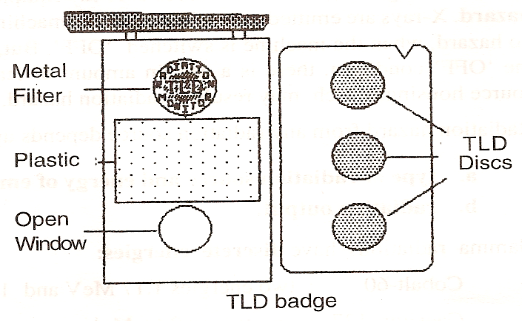
\includegraphics[width=0.5\linewidth]{TLDDosimeter.png}
            \captionof{figure}{Nanophosphors being used in TLD badges\cite{u10}}\label{fig:TLDDosimeter}
        \end{Figure}

        \begin{itemize}
            \item \textbf{Enhanced Sensitivity: } Nanophosphors possess a high surface-to-volume ratio due to 
            their small size, resulting in increased sensitivity to radiation. This enhanced sensitivity 
            allows for precise and accurate measurements of radiation doses, even at low levels.
    
            \item \textbf{Stability and Retention: } Nanophosphors are known for their long-term stability 
            and low fading rates, which ensures the reliability of dose measurements over time. They can 
            retain the stored energy and exhibit thermoluminescence or optically stimulated luminescence 
            properties, allowing for subsequent readout and analysis.

            \item \textbf{Size-Tunable Properties: } The size of nanophosphors can be precisely controlled 
            during synthesis, allowing tailoring of their optical and luminescent properties. By manipulating 
            the nanoparticle size, the emission wavelength and intensity can be tuned to match specific 
            dosimetry requirements.

            \item \textbf{Tissue-Equivalent Properties: } Some nanophosphors have tissue-equivalent 
            characteristics, meaning they exhibit similar radiation response to human tissues. This 
            property is crucial in medical dosimetry, where accurate measurement of radiation doses 
            delivered to different tissues is essential.

            \item \textbf{Multifunctionality: } Nanophosphors can be functionalized with various coatings or 
            surface modifications, enabling additional functionalities. For example, they can be embedded in 
            polymeric matrices to form composite dosimeters with enhanced mechanical properties. Nanophosphors 
            can also be conjugated with targeting molecules for specific applications, such as targeted 
            radiation therapy.
    
            \item \textbf{Real-Time Monitoring: } The small size and compatibility of nanophosphors with 
            different matrices facilitate their integration into real-time monitoring systems. They can be 
            incorporated into sensors or wearable devices, providing continuous monitoring of radiation 
            exposure in various environments.

        \end{itemize}
\end{document}











